\section{Behavioural Changes}
Overall, participants fall evenly between whether they changed their behavior after the experiment. In terms of personal informatics, many papers talk about the abundance of data that’s available to users but the lack of what to do with the data. Some papers begin to talk about what users do with information once they’ve done statistical analysis on their behavior or if that analysis is done for them and presented in a simple statement. The question asked as a result is what people do with these correlations and if these correlational statements lead to behavioral change. 

%\begin{figure}[!t]\centering
%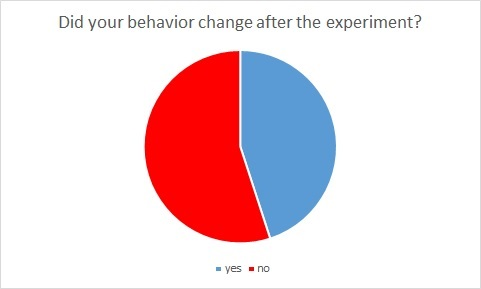
\includegraphics[width=1.0\columnwidth]{images/behavior_change.jpg}
%\caption{\footnotesize Behavioural changes by participant group after the study \label{fig:behaviorchange} 
%}
%\end{figure}

    Most researchers hypothesize that often acknowledging and making these behaviors known lead to behavioral changes. Furthermore, it is believed that reflection upon a user\textquotesingle s behavior also leads to changes. When asked if their behaviors changed after performing the experiment, those who said yes were asked to specify, and most of them state that they observed a certain behavior or noticed something new which led them to change their behavior which coincides exactly to what researchers found in the past. 
    The next question that should be asked is why people decided not to change their behavior after doing this experiment. For this set of data specifically, some of the information might shed light on why a little more than half of the participants decided not to change their behavior. There are three main reasons why we believe they might not have made behavioral changes:
    \subsection{No significant result found}
    For many participants, due to the short amount of time the experiment was run, many factors had effects on their experiment which contributed to the lack of statistical significance when attempting to prove their hypothesis. Therefore because their results were inconclusive, they have no reason to make changes to their behavior.
    \subsection{Hypothesis did not have clear cut good or bad behavior}
    For a couple of the participants, their hypothesis did not test a necessarily \enquote*{bad} behavior that they might want to change. For example, a participant tested whether apple vinegar affected their pH level. Another example is a participant who experimented with how much hot beverage she drank during the day depending on the temperature. These experiments don’t have a good or bad behavior associated with them and therefore does not call for behavioral change. 
    \subsection{No motivation to change}
    Finally, even if a participant found statistically significant results they might not believe that change is worth making other sacrifices. For experimental results to have an effect on a participant to elicit behavioral change, it must be significant to them. For example, one participants experiment asked what types of food affected him to the point of making them sick or greatly decreasing their mood. In this case it is of great value for the participant to change their behavior. On the contrary, if participants found significant results such as running increased sleep quality, perhaps running got in the way of more time of doing work or studying and so the participant believed that the opportunity cost of running for better sleep was not worth sacrificing time to do work. 
